\section{Processing of Pain in the Nervous System} \label{sec:pain}

%The International Association for the Study of Pain has presented the following definition of pain: \textit{“Pain is an unpleasant sensory and emotional experience associated with actual or potential tissue damage, or described in terms of such damage”}. \cite{1} 
Pain is a complex subjective phenomenon, where sensory and affective components along with cognitive elements are activated to refrain an individual from further and future similar damage \cite{Davis2017}. \\
When the body is exposed to a noxious stimulus, whether it originates from external or internal afflictions, information about the damaging stimulus is transmitted through neural pathways and through the peripheral nervous system to the autonomic and central nervous system. This relay to the brain of a damaging event is called nociception. It is mediated by certain receptors called nociceptors, which are attached to myelinated A$\delta$ and unmyelinated C fibers that terminate at the dorsal horn of the spinal cord. Perception of pain occurs when stimulation of nociceptors is high enough to activate A$\delta$ fibers, which results in an acute experience of prickling pain. When the stimulation increases, C fibers are activated, which results in a more intense pain experience that remains after the stimulus has ceased. These two phases of pain experience are associated with acute noxious stimulus, where the first phase is referred to as fast pain, and is of moderate intensity and appears immediately after the stimulus. The second phase, which is known as slow pain, is not as localizable, appears after a longer delay and is more painful. Activation of nociceptors can happen from sufficiently intense mechanical, chemical or thermal stimulation. Nociceptor activation is also modulated by inflammatory and bio-molecular influences. However, it is also possible for individuals to experience pain without being exposed to a measurable noxious stimulus and for individuals to undergo a damaging trauma without suffering any pain sensation. \cite{Garland2013} \\ 
As stated in The International Association for the Study of Pain’s definition of pain, not only somatosensory components are involved in the experience of pain, but also cognitive and emotional elements. Psychological processes are major elements in the perception and expression of pain and involve the individual’s attention to the painful infliction, the cognitive appraisal of pain and emotional and behavioral reactions. These factors may have increasing or decreasing effects on the perception of pain. \\
As mentioned, the activation of nociceptors is transmitted along axons in peripheral nerves to the dorsal horn of the spinal cord. From here the information ascends through the spinal cord via the spinothalamic tract to the thalamus. The thalamus functions as a major transmission location for sensory information to the cerebral cortex. The neural pathways terminate in subdivisions of the thalamic nuclei, from where the information is relayed to different cortical and subcortical divisions, including regions of the cerebral cortex, amygdala, hypothalamus, periaqueductal grey and basal ganglia. Worth remarking is that the insular cortex and cingulate cortex seem to almost always be activated when nociceptors are stimulated. \cite{Davis2017, Tracey2007} \Figref{fig:back:brain} depicts the anatomy of pain pathway propagation of neurological signal from nociceptor to spinal cord to the brain centers affiliated with pain reception and modulation.

\begin{figure}[H]                 
	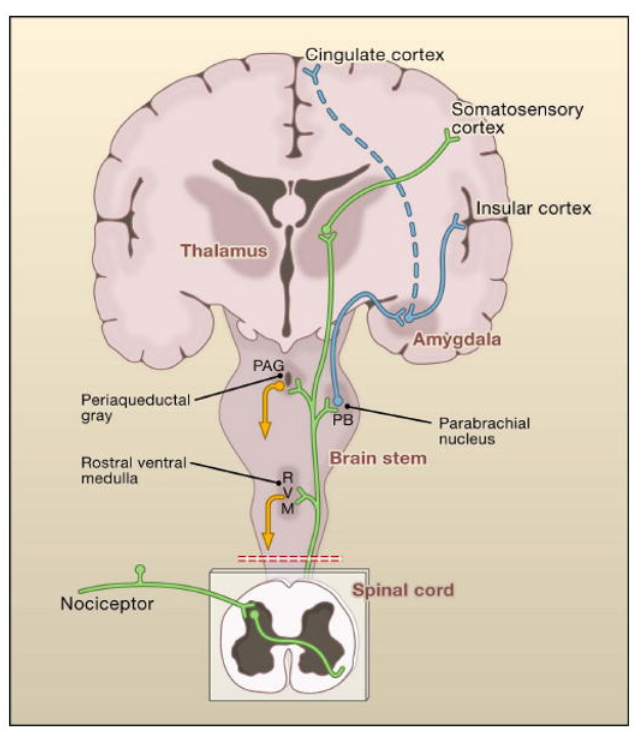
\includegraphics[width=.47\textwidth]{figures/aBackground/Brain}  
	\caption{Coronal view of the mechanisms and regions associated with the experience of pain. The anatomical pain pathway from nociceptive input propagating through the dorsal horn ascending through the spinal cord to the affiliated brain regions. Illustration taken from \cite{Basbaum2009}.}
	\label{fig:back:brain} 
\end{figure}

These regions are what process somatosensory input and is outputting neural activation that affects nociception and pain perception. \cite{Garland2013} This means that the brain does not only passively receive sensory input, but in addition actively regulates the sensory transmission by influencing the dorsal horn of the spinal cord through a descending modulation. The brain regions involved in this regulation include the same as mentioned along with the rostral ventromedial medulla and dorsolateral pons/tegmentum. \cite{Tracey2007} Thus, when determining the intensity of pain perception during noxious stimulus of an individual these brain regions are of great importance to examine. 
